% Appendix A

\chapter{OUTPUT UI}
The Output UI is the most important component that provides the interface between this system and the user. And so, all the possible outputs of this module needs explaining. 

\section{SAFE WEBSITE}
As most of the sites that will be visited by a user will be safe, unless the search engine that the user uses has been compromised. The above holds good statistically. And, in the Figure  ~\ref{fig:ahtmlc}, the Output UI for the official university website is shown.

\begin{figure}[htp]
\centering
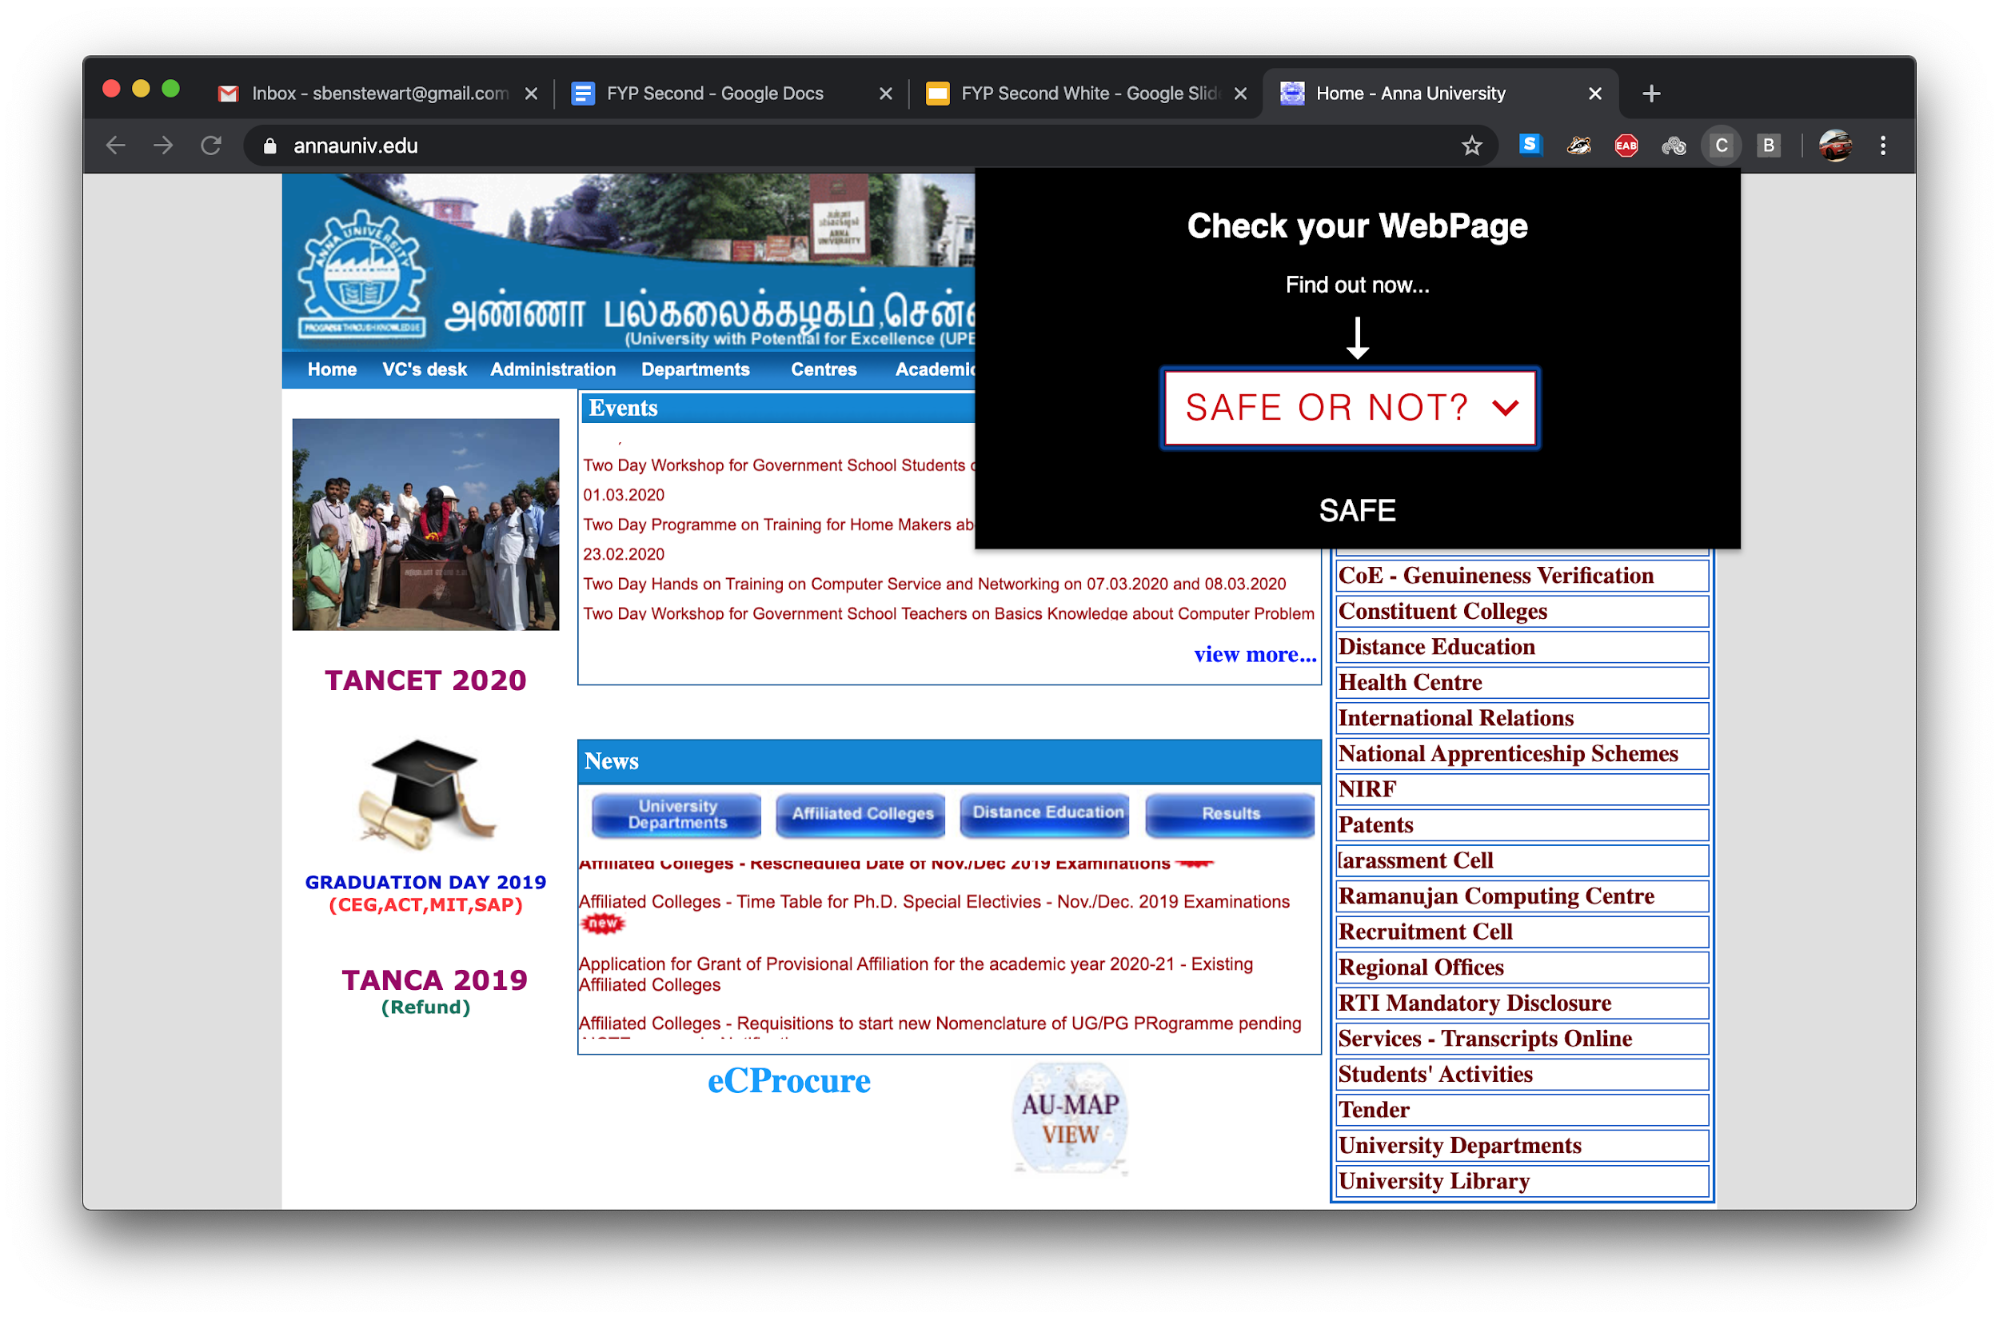
\includegraphics[scale=0.2]{Figures/image2.png}
\caption{SAFE Website}
\label{fig:ahtmlc}
\end{figure}

\section{PHISHING WEBSITE}
This type of websites make the smallest part of websites that the user visits. There are multiple different outputs possible for this scenario, which will be discussed in detail.

\subsection{CORRECT PHISH DETECTION AND CORRECT TARGET IDENTIFICATION}
The phish detector finds the phish correctly, and the target detector which displays the most closely related site is the same website that the phish is based on. This is shown in the Figure ~\ref{fig:cc}, where the phish website impersonates Twitter, which both the phish detector and target identifier find correctly.

\begin{figure}[htp]
\centering
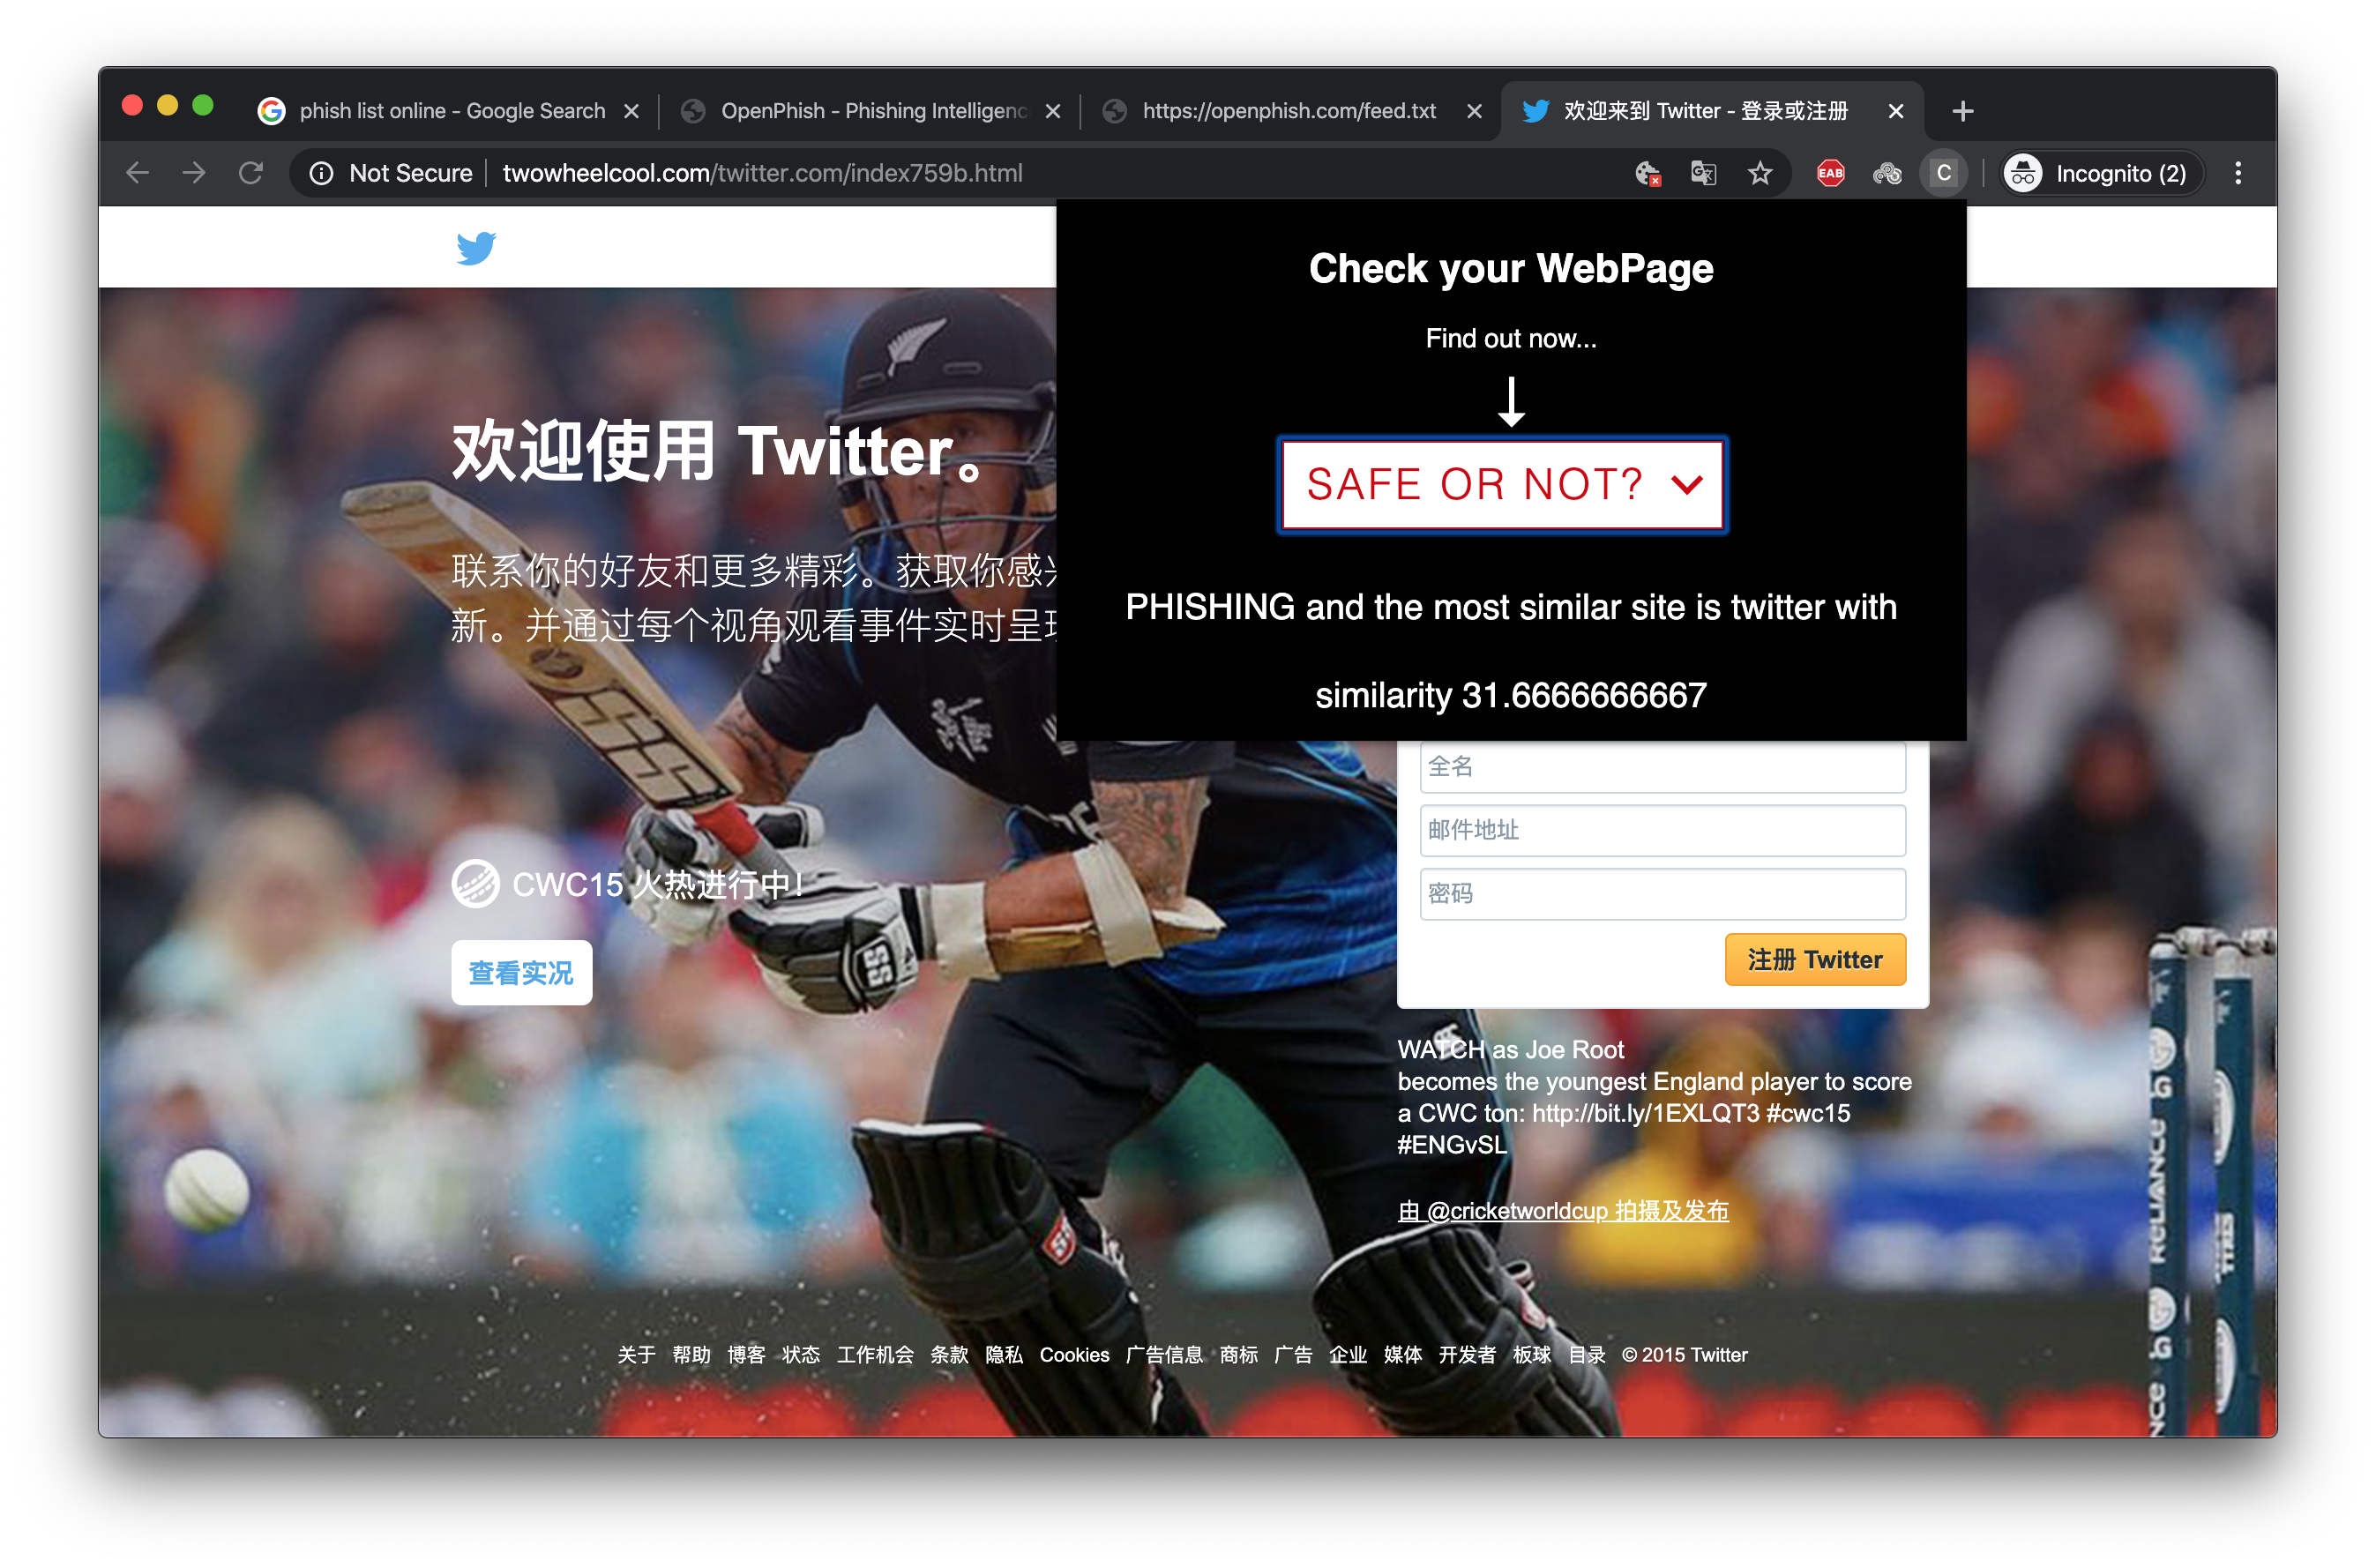
\includegraphics[scale=0.2]{Figures/image17.png}
\caption{Correct Phish Detection and Correct Target Identification}
\label{fig:cc}
\end{figure}

\subsection{CORRECT PHISH DETECTION AND INCORRECT TARGET IDENTIFICATION}
The phish detector finds the phish correctly, but the target detector which displays the most closely related site is not the same website that the phish is based on. This is shown in the Figure ~\ref{fig:ci}, where the phish website impersonates FaceBook, but the target identifier could not classify it.

\begin{figure}[htp]
\centering
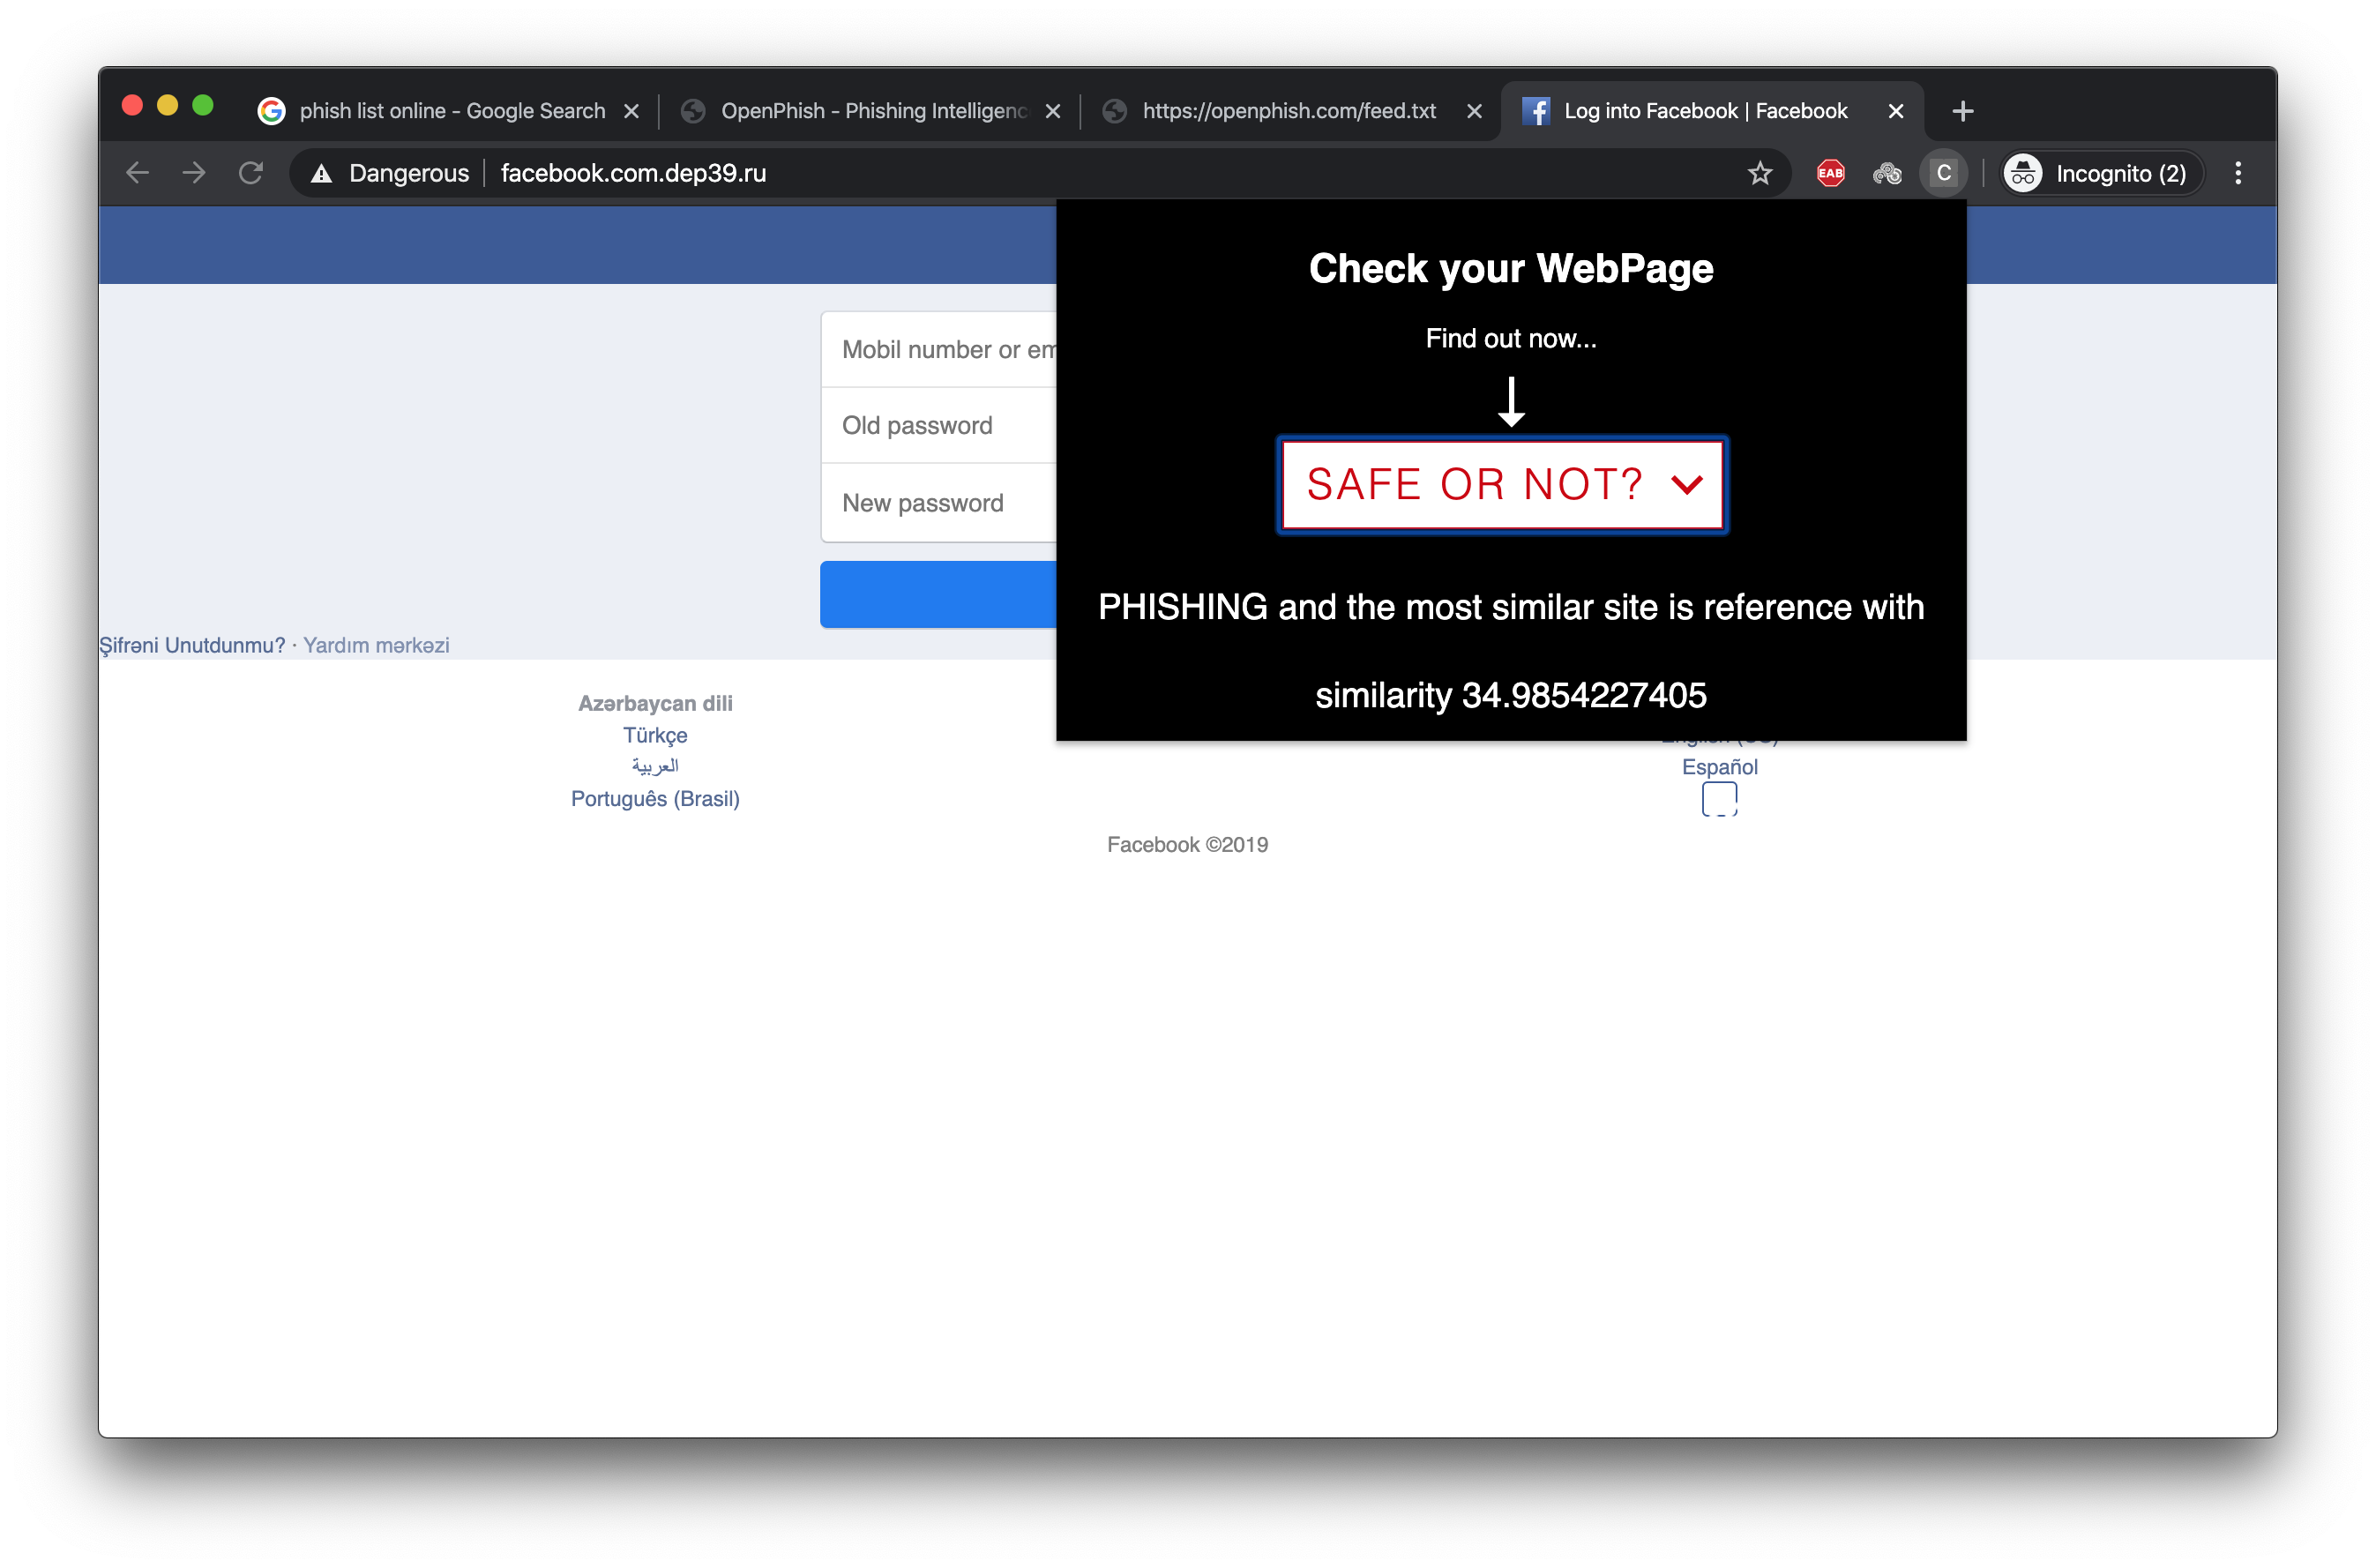
\includegraphics[scale=0.2]{Figures/image18.png}
\caption{Correct Phish Detection and Incorrect Target Identification}
\label{fig:ci}
\end{figure}

\subsection{INCORRECT PHISH DETECTION}
The phish detector finds the phish incorrectly. This is a problem, and so the model has been skewed so that the incorrect classifications will be only where the safe websites are incorrectly classified as phish. Figure ~\ref{fig:i} shows the instance where the phish detector incorrectly classifies the personal website of S.Ben Stewart who worked on this system as a phish. The future work involves rooting out cases like this.

\begin{figure}[htp]
\centering
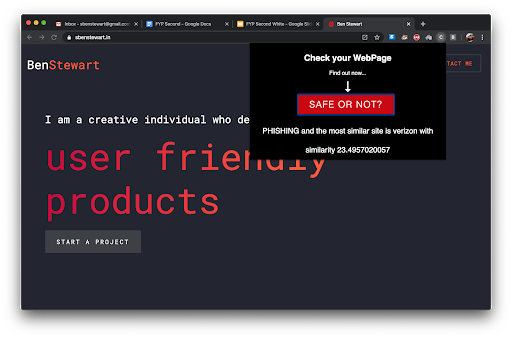
\includegraphics[scale=0.5]{Figures/image19.png}
\caption{Correct Phish Detection and Incorrect Target Identification}
\label{fig:i}
\end{figure}

